{\fontsize{12pt}{22pt} \textbf{Correlation}\par}

\vspace{5mm}

\underline{Pearson coefficient}:

\begin{center}
$\rho_{X,Y} = \frac{cov(X,Y)}{\sigma_X \sigma_Y}$
\end{center}

\textit{np.cov(a,b)} gives a \textbf{matrix} with covariances and \textbf{unbiased} variances (on the diagonal). 

Several computation equivalences are shown below:

\lstset{language=Python}
\lstset{frame=lines}
\lstset{caption={Pearson coefficient replication}}
\lstset{label={lst:code_direct}}
\lstset{basicstyle=\footnotesize}
\begin{lstlisting}

a = pd.Series([5, 2, 6])
b = pd.Series([18, 2, 5])

print(a.corr(b) # biased standard deviation estimators !!
      == np.corrcoef(a,b)[0,1] 
      == (np.cov(a,b)[0,1] / np.sqrt(np.cov(a,b)[0,0]*np.cov(a,b)[1,1]))
      == np.cov(a,b)[0,1] / (np.std(a,ddof=1)*np.std(b,ddof=1)) 
      != np.cov(a,b)[0,1] / (np.std(a)*np.std(b)))

# prints True

\end{lstlisting}

\vspace{5mm}

\textit{Note}: when we compute those statistics numerically, we use \textbf{empirical} values.

Thus, $\mathbb{V}[X] = \mathbb{E}[X-\mathbb{E}[X]]$ is computed as $var_n(x)=\frac{1}{n}\Sigma(x_i - \overline{x})^2$

\vspace{5mm}

\underline{Autocorrelation (1)}:

\begin{center}
$R_{k} = \frac{\mathbb{E}[(X_i-\mu_X)(X_{i+k}-\mu_X)]}{\sigma_X^2}$
\end{center}

$X_i$ is the dataset without the last $k$ values

$X_{i+k}$ is the dataset without the first $k$ values

$\mu_X$ is the mean on \textbf{the whole} dataset $X$

$\sigma_X^2$ is the variance \textbf{the whole} dataset $X$

\vspace{5mm}

\underline{Autocorrelation (2)}:

\begin{center}
$R_{k} = \frac{\mathbb{E}[(X_i-\mu_{X_i})(X_{i+k}-\mu_{X_{i+k}})]}{\sigma_{X_i}\sigma_{X_{i+k}}}$
\end{center}

$X_i$ is the dataset without the last $k$ values

$X_{i+k}$ is the dataset without the first $k$ values

$\mu_{X_i}$ is the mean on dataset $X_i$

$\sigma_{X_i}$ is the standard deviation on dataset $X_i$

\vspace{5mm}

\textit{statsmodels.tsa.stattools.acf} uses formula (1).

\textit{np.autocorr} uses formula (2).

Below is the summary of equivalences:

\lstset{language=Python}
\lstset{frame=lines}
\lstset{caption={Autocorrelation replication}}
\lstset{label={lst:code_direct}}
\lstset{basicstyle=\footnotesize}
\begin{lstlisting}

import statsmodels.tsa.stattools as sm

s = pd.Series([5, 2, 6, 18, 2, 5])

a = pd.Series([5, 2, 6])
b = pd.Series([18, 2, 5])

# Formula (1)
print(s.autocorr(3) # unbiased standard deviation estimators !!
      == a.corr(b)
      ==  np.cov(a,b)[0,1]/(np.std(a,ddof=1)*np.std(b,ddof=1)))

# prints True

# Formula (2)
def acf_by_hand(x, lag):
    y1 = np.array(x[:(len(x)-lag)])
    y2 = np.array(x[lag:])
    sum_product = np.sum((y1-np.mean(x))*(y2-np.mean(x)))
    return sum_product / (len(x) * np.var(x))

print(round(acf_by_hand(s,3),6)
        == round(sm.acf(s)[3],6)) # biased covariance and standard deviation estimators !!

# prints True

\end{lstlisting}

\vspace{5mm}

Below a graphical comparison of both formulas:

\lstset{language=Python}
\lstset{frame=lines}
\lstset{caption={Graphical comparison of correlation computations}}
\lstset{label={lst:code_direct}}
\lstset{basicstyle=\footnotesize}
\begin{lstlisting}

import statsmodels.tsa.stattools as sm

s = pd.Series([5, 2, 6, 18, 2, 5])
a = pd.Series([5, 2, 6])
b = pd.Series([18, 2, 5])

corr_statsmodel =  sm.acf(s)[1:4]
corr_pandas = [s.autocorr(i) for i in range(1,4)]

test_df = pd.DataFrame([corr_statsmodel, corr_pandas]).T
test_df.columns = ['Pandas Autocorr', 'Statsmodels Autocorr']
test_df.index += 1
test_df.plot(kind='bar')

\end{lstlisting}

\begin{center}
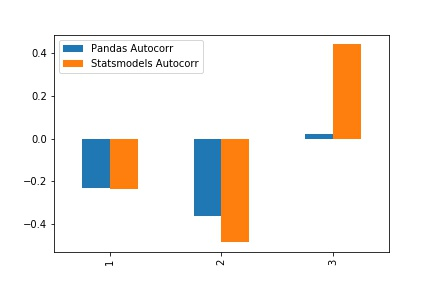
\includegraphics[scale=0.6]{corr_comparison.jpg}
\end{center}

\vspace{5mm}

\underline{Partial autocorrelation}

\vspace{5mm}

Based on article \href{https://towardsdatascience.com/understanding-partial-auto-correlation-fa39271146ac}{understanding-partial-auto-correlation (towardsdatascience)}

\vspace{5mm}

\begin{center}
$PR_k = \frac{cov(X_t | X_{t-1} ... X_{t-k+1},X_{t-k} | X_{t-1} ... X_{t-k+1})}{\sigma_{X_t | X_{t-1} ... X_{t-k+1}} \sigma_{X_{t-k} | X_{t-1} ... X_{t-k+1}}}$
\end{center}

$X_t | X_{t-1} ... X_{t-k+1}$ is the residual of regression $X_t = \beta_0 + \beta_1 X_{t-1} + ... + \beta_k X_{t-k+1}$

$X_{t-k} | X_{t-1} ... X_{t-k+1}$ is the residual of regression $X_{t-k} = \beta_0 + \beta_1 X_{t-1} + ... + \beta_k X_{t-k+1}$

\vspace{5mm}

Thus, one can write:

\begin{center}
$PR_k = \rho_{\epsilon_t,\epsilon_{t-k}}$
\end{center}

\vspace{5mm}

We use partial autocorrelation in order to define the order $p$ in which we can compute an AR(p) model.

\begin{center}
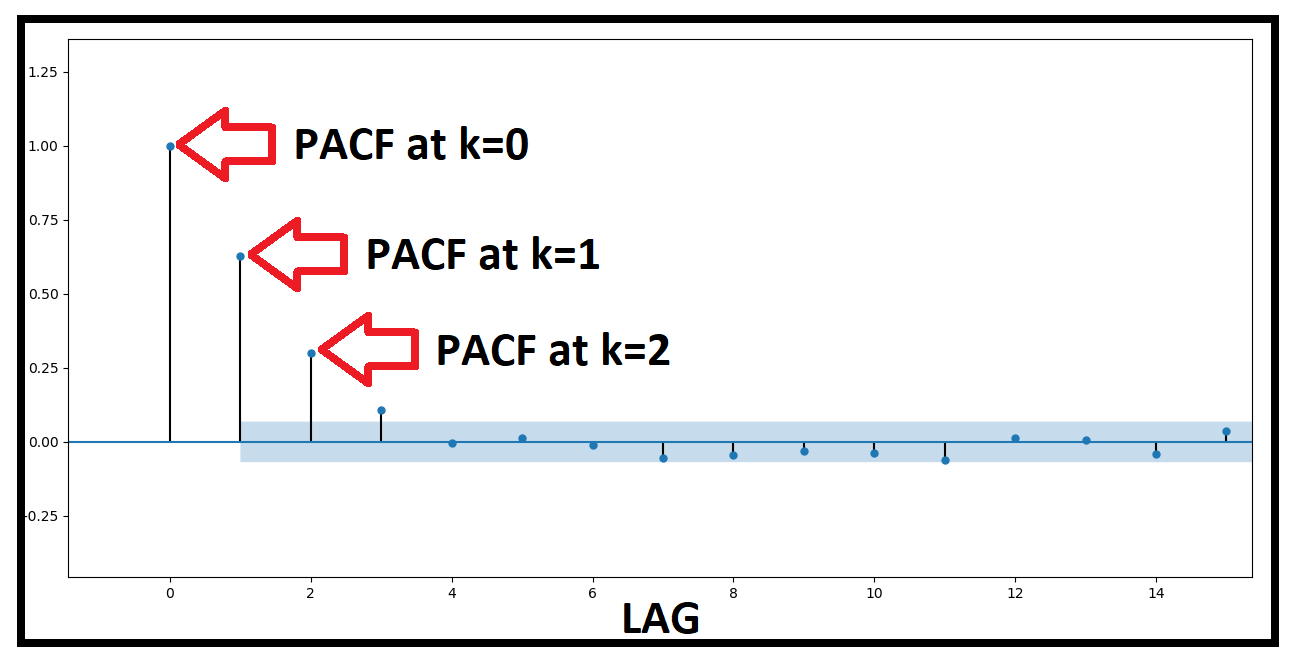
\includegraphics[scale=0.2]{PACF.png}
\end{center}

\vspace{5mm}

Based on this graph, we can use an AR(2) or even AR(3) ($k=3$ is just outside the 95\% confidence interval.

\vspace{5mm}
